\chapter{Project context}
    %\addcontentsline{toc}{chapter}{}
My project was In the occasion of a summer internship . In the rest of this chapter i will present my host organisation and Then i will explain the main idea and the purpose of my application.  
\section{Company presentation}
\subsection{Company Description}
Mind Engineering is an agency specializing in the design of innovative , efficient and customized software solutions . They are a team of developers, designers and project managers, all experts, passionate about thei	r business and proud of the solutions they offer to their partners.
\subsection{Accomplishements}
Mind engineering had achieved too much success in a very limited period . They have a completed many successful projects since their beginning in 2015 until now  and 
these are some examples : 
\begin{itemize}
\item ISTIC website : 
\begin{figure}[H]
	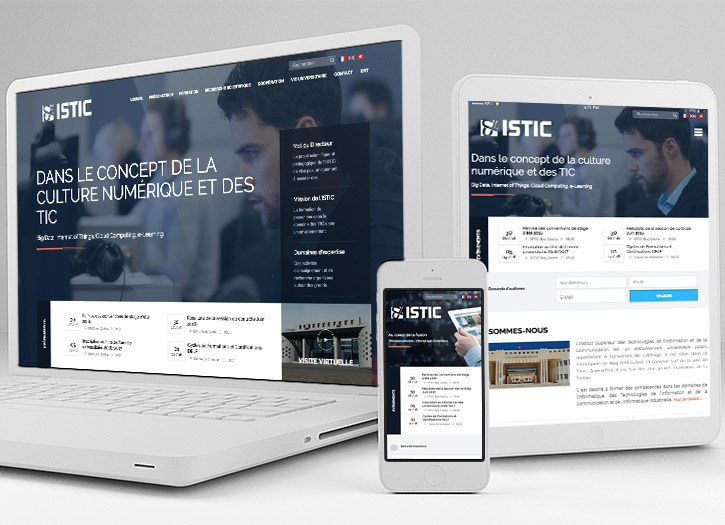
\includegraphics[width=10cm]{istic.jpg}
		\caption{\href{http://www.istic.rnu.tn/}{www.istic.rnu.tn} : ISTIC Website}
	\label{istic website}
\end{figure}



\item SOGEFEC (Societe generale froid et climatisation) website : 
\begin{figure}[H]
	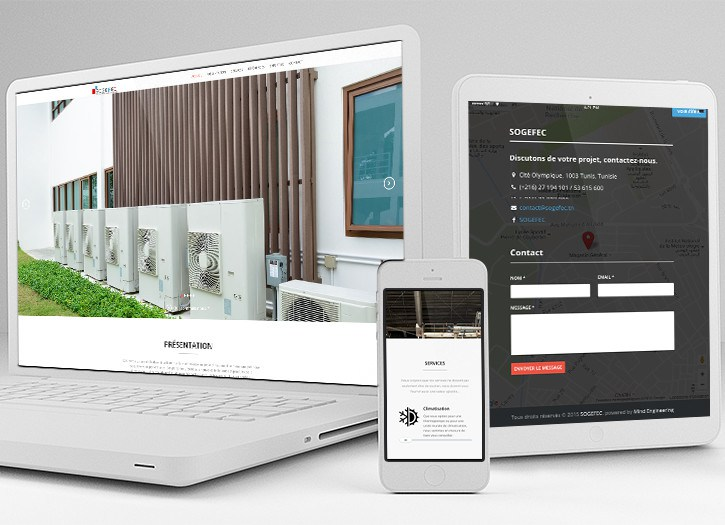
\includegraphics[width=10cm]{sogefec.jpg}
	\caption{\href{http://www.sogefec.tn/}{http://www.sogefec.tn/}  sogefec website}
	\label{istic website}
\end{figure}

\item Jadal online  : 
\begin{figure}[H]
	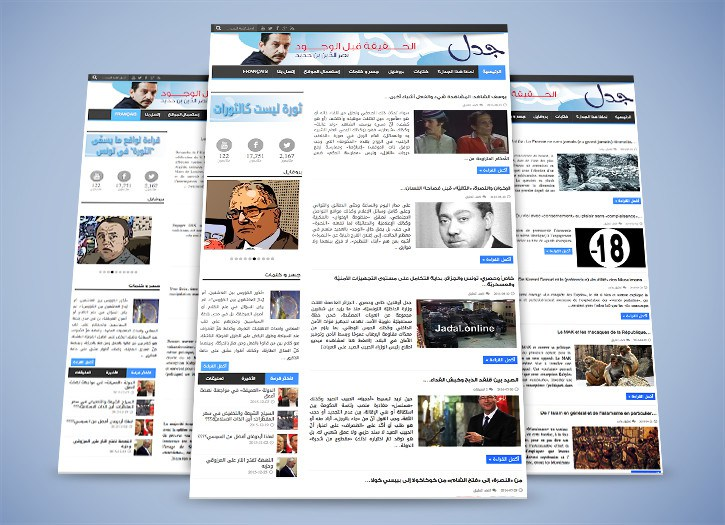
\includegraphics[width=10cm]{jadal.jpg}
	\caption{\href{http://jadal.online/}{http://jadal.online/}  jadal online}
	\label{istic website}
\end{figure}


\end{itemize}


\newpage
\section{Application context}
In this section we will discuss the main purpose of the application . and why every news website should build it's own mobile app . 
\subsection{The noticed rise of mobile devices users and internet users }
The report from the National Telecommunication Forum (INT), published on its website, Tunisians are using a 3G compatible phone, 23.5 percent change their phone every 6 months and 60 percent spend more than 3 hours a day online, against 36 percent between 1 and 3 hours a day and 12 percent within an hour  day.

\subsection{The migration to android }
According to GSM Arena Android will be the most popular mobile OS in the next four years reaching almost 50 percent market share. Meanwhile Windows Phone will catch up and overtake the second place from iOS by 2015 with 20 percent market share.
\subsection{Advantages from using mobile apps for news websites }
Firstly using a mobile app to browse news will create a very good user experience for website followers since mobile apps are very handy and portable which will make the users feel connected and updated with the latest news  . and never forget the simplicity of smartphones using ( it usually takes two or three taps to open the application).
\\*
\\Secondly , Using a mobile app to browse news is economic since you will only require the data and then the application will care for parsing these data , processing them and making show them to the user which will optimize your mobile data using and optimize responding time from the server since we are not requiring extra additional things from the website server like i html , css , javascrit ...etc in websites.
\\*
\\Last but not least , The mobile push notification service is a very useful webservice for news websites  since it offers the possibility for the users to be instantly updated with latest breaking news . 
 \subsection{conclusion}
 To conclude , the current market circumstances and the various advantages of building your news mobile app aside to your apps imposes the necessity of odopting this solution.
 \\Added to that the huge migration to android platforms will make every person think of creating an android app before any other platform .   


